\documentclass[margin=0.5cm]{standalone}

\usepackage{tikz}
\usepackage{newtxtext}
\usepackage{newtxmath}
\usepackage{xcolor}

\definecolor{starfishyellow}{HTML}{FFBD59}
\definecolor{starfishblue}{HTML}{004AAD}

\begin{document}

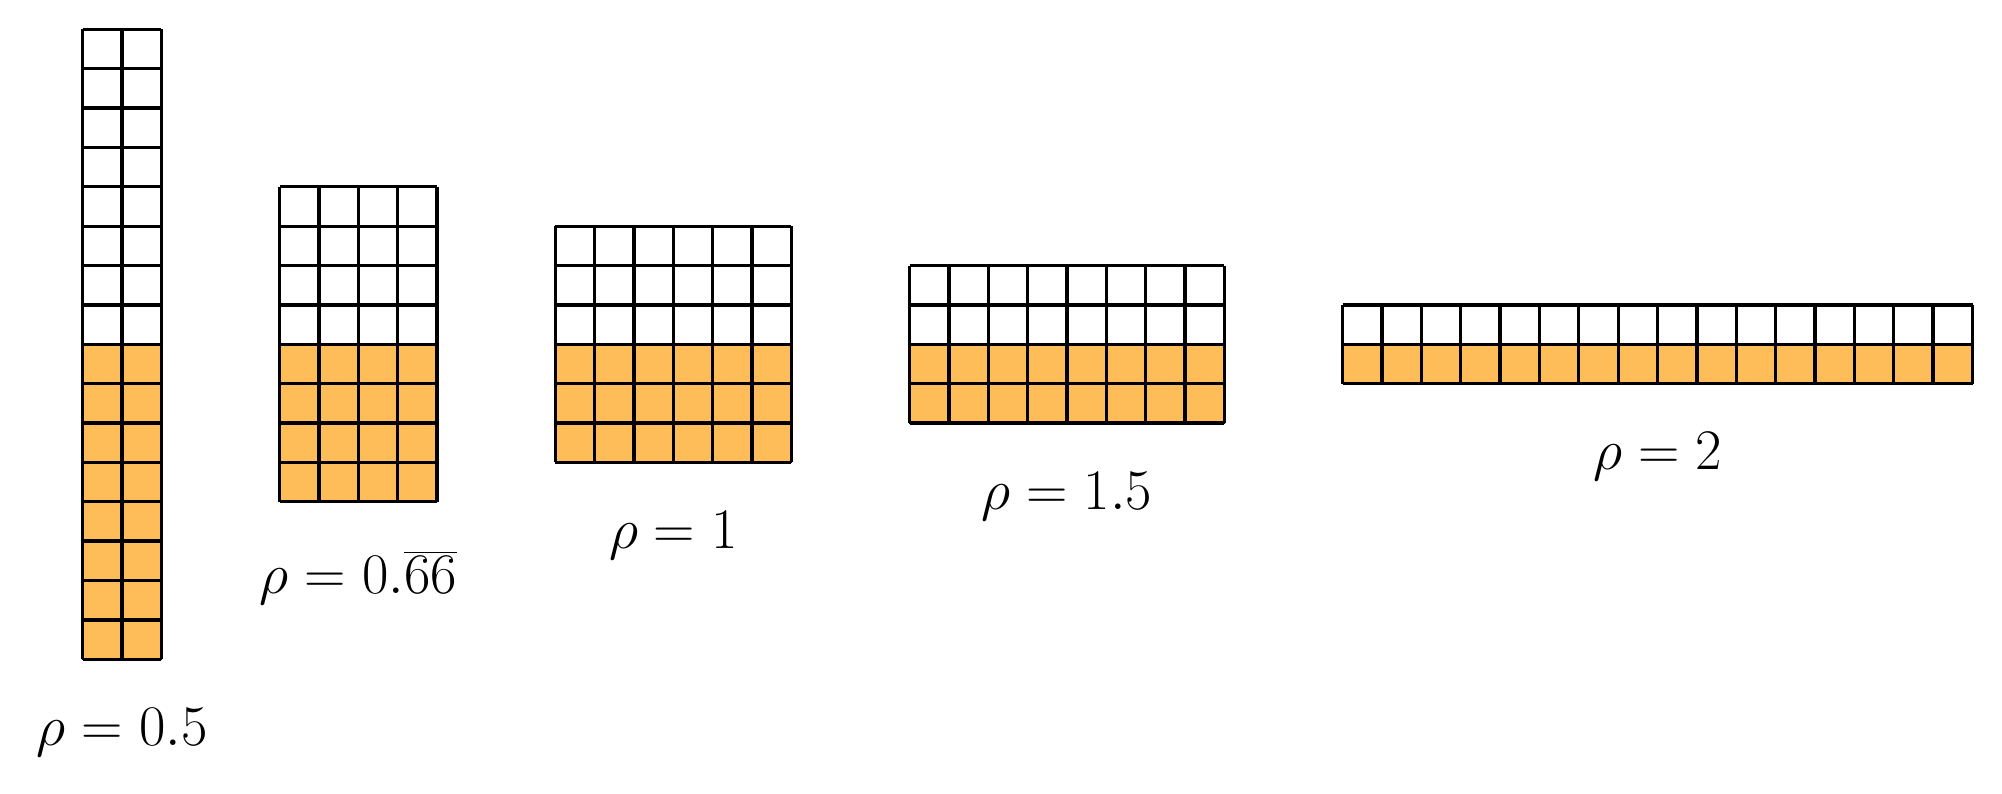
\begin{tikzpicture}
  \draw[fill=starfishyellow] (-7.5,-4.0) rectangle (-6.5,0.0);
  \draw[step=0.5cm,black,very thick] (-7.5,-4.0) grid (-6.5,4.0);
  \node[anchor=north] at (-7.0, -4.5) {\huge $\rho = 0.5$};


  \draw[fill=starfishyellow] (-5.0,-2.0) rectangle (-3.0,0.0);
  \draw[step=0.5cm,black,very thick] (-5.0,-2.0) grid (-3.0,2.0);
  \node[anchor=north] at (-4.0, -2.5) {\huge $\rho = 0.\overline{66}$};


  \draw[fill=starfishyellow] (-1.5,-1.5) rectangle (1.5,0.0);
  \draw[step=0.5cm,black,very thick] (-1.5,-1.5) grid (1.5,1.5);
  \node[anchor=north] at (0, -2.0) {\huge $\rho = 1$};


  \draw[fill=starfishyellow] (3.0,-1.0) rectangle (7.0,0.0);
  \draw[step=0.5cm,black,very thick] (3.0,-1.0) grid (7.0,1.0);
  \draw[black,thick] (3.0,-1.0) -- (3.0,1.0);
  \node[anchor=north] at (5.0, -1.5) {\huge $\rho = 1.5$};


  \draw[fill=starfishyellow] (8.5,-0.5) rectangle (16.5,0.0);
  \draw[step=0.5cm,black,very thick] (8.5,-0.5) grid (16.5,0.5);
  \draw[black,thick] (8.5,-0.5) -- (8.5,0.5);
  \node[anchor=north] at (12.5, -1.0) {\huge $\rho = 2$};
\end{tikzpicture}

\end{document}
